\documentclass[11pt,a4paper]{article}

% ── Packages ────────────────────────────────────────────────────────────────
\usepackage[utf8]{inputenc}
\usepackage[T1]{fontenc}
\usepackage[british]{babel}
\usepackage{lmodern}
\usepackage{microtype}
\usepackage{amsmath,amssymb,amsthm}
\usepackage{mathtools}
\usepackage{booktabs}
\usepackage{longtable}
\usepackage{array}
\usepackage{colortbl}
\usepackage{xcolor}
\usepackage{hyperref}
\usepackage{geometry}
\usepackage{graphicx}
\usepackage{tikz}
\usepackage{tcolorbox}
\usepackage[numbers]{natbib}
\usepackage{caption}
\usepackage{float}

\usetikzlibrary{positioning,shapes.geometric,fit,backgrounds,calc}

\geometry{a4paper, margin=2.5cm}

\hypersetup{
  colorlinks = true,
  linkcolor  = blue!60!black,
  citecolor  = blue!60!black,
  urlcolor   = blue!60!black,
  pdftitle   = {D-exp-MP01: PDL Structural Lacunae Confirmed by Materials Project},
  pdfauthor  = {Cédric Laubscher}
}

% ── tcolorbox styles ────────────────────────────────────────────────────────
\tcbuselibrary{skins,breakable}

\newtcolorbox{pdlresult}[2][]{
  enhanced, breakable,
  colback  = green!5!white,
  colframe = green!40!black,
  fonttitle= \bfseries,
  title    = {#2}, #1
}

\newtcolorbox{pdlconjecture}[2][]{
  enhanced, breakable,
  colback  = orange!5!white,
  colframe = orange!60!black,
  fonttitle= \bfseries,
  title    = {#2}, #1
}

\newtcolorbox{pdlopen}[2][]{
  enhanced, breakable,
  colback  = gray!5!white,
  colframe = gray!50!black,
  fonttitle= \bfseries,
  title    = {#2}, #1
}

\newtcolorbox{epistemicbox}{
  enhanced,
  colback  = blue!3!white,
  colframe = blue!40!black,
  fonttitle= \bfseries,
  title    = {Epistemic Status Table}
}

% ── Theorem environments ─────────────────────────────────────────────────────
\newtheorem{theorem}{Theorem}
\newtheorem{lemma}[theorem]{Lemma}
\newtheorem{proposition}[theorem]{Proposition}
\newtheorem{corollary}[theorem]{Corollary}
\theoremstyle{definition}
\newtheorem{definition}{Definition}
\newtheorem{conjecture}{Conjecture}
\theoremstyle{remark}
\newtheorem{remark}{Remark}

% ── Colours for the periodic table ──────────────────────────────────────────
\definecolor{mgcolor}{RGB}{232,228,248}   % magic number fill
\definecolor{mgbord}{RGB}{85,72,176}      % magic number border
\definecolor{thcolor}{RGB}{228,244,237}   % theorem fill
\definecolor{thbord}{RGB}{26,122,80}      % theorem border
\definecolor{lccolor}{RGB}{253,240,220}   % lacuna fill
\definecolor{lcbord}{RGB}{176,96,16}      % lacuna border
\definecolor{opcolor}{RGB}{235,235,235}   % open fill
\definecolor{opbord}{RGB}{138,138,138}    % open border
\definecolor{lacolor}{RGB}{234,244,232}   % lanthanide/actinide fill
\definecolor{labord}{RGB}{58,122,48}      % lanthanide/actinide border

% ── Title ────────────────────────────────────────────────────────────────────
\title{\textbf{D-exp-MP01: PDL Structural Lacunae Confirmed\\
by Materials Project Database Scan}\\[6pt]
{\large Exploratory Document — PDL Framework}}

\author{Cédric Laubscher\\[4pt]
\small Independent Researcher, Switzerland\\
\small \href{https://cedriclaubscher.ch}{cedriclaubscher.ch}
\and
\small \textit{PDL corpus references:}\\
\small D40~\cite{Laubscher_D40_2025},
       D47~\cite{Laubscher_D47_2025},
       DS01~\cite{Laubscher_DS01_2025}}

\date{May 2026}

% ════════════════════════════════════════════════════════════════════════════
\begin{document}
\maketitle

% ── Abstract ─────────────────────────────────────────────────────────────────
\begin{abstract}
The Projective Dynamic Logo (PDL) framework derives the valley of nuclear stability and the periodic table from four combinatorial axioms (C1--C4) acting on finite signed graphs, with zero free parameters~\cite{Laubscher_D40_2025,Laubscher_D47_2025}. Conjecture OP3 of document D40 identifies technetium ($Z=43$) and promethium ($Z=61$) as \emph{structural lacunae}: elements for which no stable nuclear configuration is possible at the Block~II (nuclear) level. We test this prediction against the Materials Project database~\cite{Jain_2013} by scanning all $Z=1$--$83$ elements and comparing the number of experimentally observed compounds (flag \texttt{theoretical=False}, energy above hull $<0.05$\,eV) per element. Technetium shows a $10.5\times$ deficit in observed compounds relative to its immediate neighbours, and promethium a $484\times$ deficit, with $z$-scores of $-2.31\sigma$ and $-5.08\sigma$ respectively against the distribution of 29 stable odd-$Z$ elements above $Z=20$. The \texttt{theoretical} flag reveals that 99.3\% of promethium's database entries are pure DFT predictions with no experimental counterpart. These results constitute a strong empirical correlation with Conjecture OP3-D40, whilst the causal mechanism connecting Block~II (nuclear stability) to Block~III (chemical richness) remains an open problem (OP4) of the PDL programme.
\end{abstract}

\tableofcontents

% ── Epistemic status ─────────────────────────────────────────────────────────
\section*{Epistemic Status}

\begin{epistemicbox}
\begin{center}
\renewcommand{\arraystretch}{1.3}
\begin{tabular}{lll}
\toprule
\textbf{Claim} & \textbf{Status} & \textbf{Reference} \\
\midrule
Magic numbers $\{2,8,20,28,50,82,126\}$ & Unconditional theorem (C1--C4) & D47~\cite{Laubscher_D47_2025} \\
$N_{\min}(Z)$ exact for $Z=1$--$82$ & Unconditional theorem (C1--C4) & D40~\cite{Laubscher_D40_2025} \\
Structural lacunae Tc, Pm & Conjecture OP3-D40 & D40~\cite{Laubscher_D40_2025} \\
MP deficit for Tc/Pm & Empirical fact (this document) & --- \\
Causal link Block~II $\to$ Block~III & Open problem OP4 & DM~\cite{Laubscher_DM_2025} \\
\bottomrule
\end{tabular}
\end{center}
\end{epistemicbox}

% ════════════════════════════════════════════════════════════════════════════
\section{Introduction}
\label{sec:intro}

The Projective Dynamic Logo (PDL) is a foundational research programme that derives physical laws and constants from four combinatorial axioms (C1--C4) on finite signed graphs, without presupposing spacetime, particles, or fields~\cite{Laubscher_DS01_2025}. At the nuclear level (Block~II of the programme), the framework produces the valley of nuclear stability and the full periodic table up to lead ($Z=82$) as unconditional theorems~\cite{Laubscher_D40_2025,Laubscher_D47_2025}.

A central result of D47~\cite{Laubscher_D47_2025} is the uniqueness theorem for the proton asymmetry $\Delta n = n_d - n_u = 4$: this is the unique admissible value for which the discriminant of the proton's structural equation is a perfect square ($149^2 = 22201$). This single integer generates a spin-orbit splitting $s = \Delta n / 2n_u = 1/12$, which reproduces exactly the seven nuclear magic numbers without any free parameter.

Among the 82 stable elements, Conjecture OP3 of D40~\cite{Laubscher_D40_2025} identifies two \emph{structural lacunae}: technetium ($Z=43$) and promethium ($Z=61$), the only two elements below bismuth with no stable isotope in nature. The conjecture states that no collective surface closure is possible for any neutron number $N$ at these values of $Z$. This prediction, derived from purely combinatorial considerations, admits an independent empirical test against chemical databases.

The Materials Project~\cite{Jain_2013} is a high-throughput computational materials science platform providing density functional theory (DFT) data for $\sim$160\,000 inorganic materials. A key metadata flag, \texttt{theoretical}, distinguishes between structures that have been experimentally observed and those that are purely computational predictions. This distinction maps naturally onto the PDL prediction: if Tc and Pm cannot form stable nuclear configurations, they should leave a measurable signature in the chemical record.

% ════════════════════════════════════════════════════════════════════════════
\section{PDL Background}
\label{sec:pdl}

\subsection{Axioms and the proton quintuplet}

The four axioms C1--C4 act on finite signed graphs. C1 (binary pulsation) requires each edge to oscillate between active and inactive states. C2 (triangular coherence) requires every triangle to have a positive product of signed edges. C3 (minimal completeness) selects the smallest closed structure satisfying C1--C2. C4 (logical optimisation) minimises internal conflict.

The unique minimal structure satisfying C1--C4 is the complete graph $K_4$ on four vertices. Assembling $K_4$ units into a hierarchical structure carrying net charge $+1$ yields a single integer solution: the \emph{proton quintuplet}
\begin{equation}
  (n_u,\, n_d,\, r_{\mathrm{val}},\, R_{\mathrm{sea}},\, R_{\mathrm{tot}})
  = (24,\, 28,\, 930,\, 10087,\, 11017).
  \label{eq:quintuplet}
\end{equation}

\subsection{Uniqueness of \texorpdfstring{$\Delta n = 4$}{Delta n = 4} and the magic numbers}

The asymmetry $\Delta n = n_d - n_u = 4$ satisfies the structural equation
\begin{equation}
  3\,n_u^2 + (2\Delta n - 3)\,n_u + \Delta n(\Delta n - 1) - 2 r_{\mathrm{val}} = 0,
  \label{eq:struct}
\end{equation}
whose discriminant is a perfect square if and only if $\Delta n = 4$, yielding $\mathrm{disc} = 149^2 = 22201$. This is the \emph{uniqueness theorem} of D47~\cite{Laubscher_D47_2025}.

The spin-orbit splitting
\begin{equation}
  s = \frac{\Delta n}{2\,n_u} = \frac{4}{48} = \frac{1}{12}
  \label{eq:splitting}
\end{equation}
depresses the maximal-$j$ sub-shells of the nuclear harmonic oscillator, generating the seven magic numbers $\{2,8,20,28,50,82,126\}$ as an unconditional theorem~\cite{Laubscher_D47_2025}.

\subsection{Valley of stability and structural lacunae}

The minimum neutron number for nuclear stability is derived as (D40):
\begin{equation}
  N_{\min}(Z) = \begin{cases}
    Z & Z \leq Z_{\mathrm{sat}} = 20, \\
    20 + \displaystyle\sum_{Z'=22,24,\ldots,Z} r_{\mathrm{exc}}(Z') & Z > 20,
  \end{cases}
  \label{eq:nmin}
\end{equation}
where $r_{\mathrm{exc}}(Z') = 0$ if $Z' \in \{28,50,82\}$ and $r_{\mathrm{exc}}(Z')=1$ otherwise. The formula reproduces $N_{\min}(Z)$ exactly for all $Z = 1$--$82$ with zero free parameters~\cite{Laubscher_D40_2025}.

\begin{pdlconjecture}{Conjecture OP3-D40 (Structural Lacunae)}
For $Z=43$ (technetium) and $Z=61$ (promethium), no collective surface closure is admissible for any neutron number $N$. These elements cannot possess a stable isotope within the PDL Block~II framework.
\end{pdlconjecture}

\clearpage
% ════════════════════════════════════════════════════════════════════════════
\section{The PDL Periodic Table}
\label{sec:table}

Figure~\ref{fig:ptable} presents the periodic table annotated by PDL epistemic status. The colour coding distinguishes four categories: magic numbers (purple, unconditional theorem), stable elements $Z\leq82$ (green, theorem), structural lacunae (amber, conjecture OP3), and elements beyond Pb (grey, open problem OP15).

% ── TikZ Periodic Table ───────────────────────────────────────────────────
\begin{figure}[H]
\centering
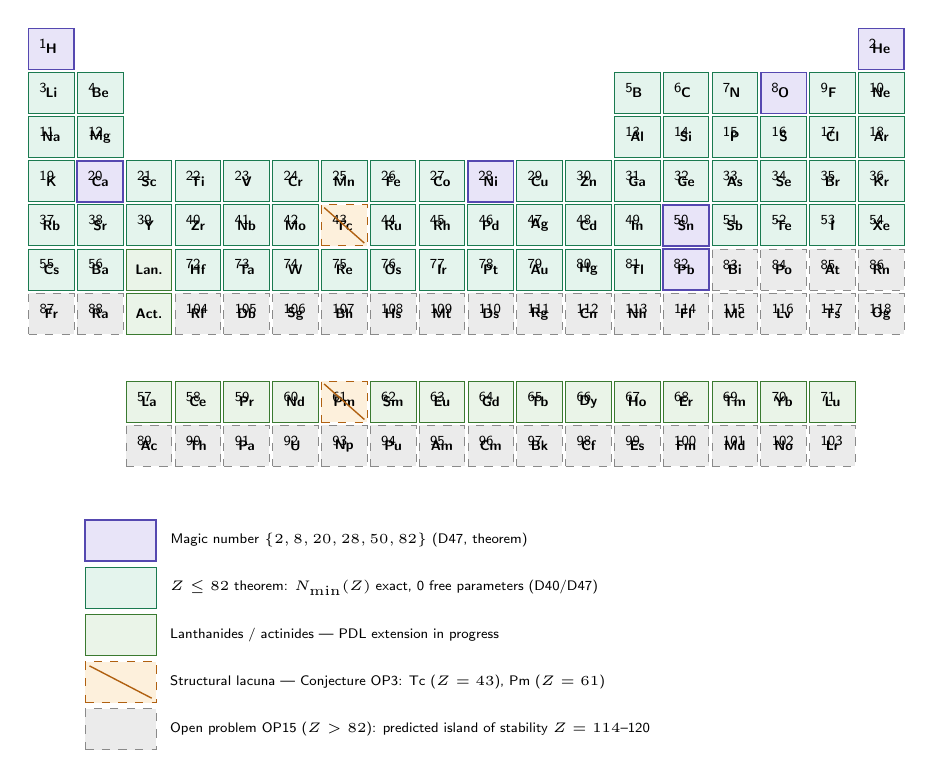
\begin{tikzpicture}[
  pdlcell/.style={
    rectangle, minimum width=0.58cm, minimum height=0.52cm,
    inner sep=0pt, font=\fontsize{4.2}{5}\selectfont\sffamily
  },
  pdlmg/.style={pdlcell, fill=mgcolor, draw=mgbord, line width=0.6pt},
  pdlth/.style={pdlcell, fill=thcolor, draw=thbord, line width=0.3pt},
  pdllc/.style={pdlcell, fill=lccolor, draw=lcbord, line width=0.3pt, dashed},
  pdlop/.style={pdlcell, fill=opcolor, draw=opbord, line width=0.25pt, dashed},
  pdlla/.style={pdlcell, fill=lacolor, draw=labord, line width=0.25pt},
  pdlznum/.style={font=\fontsize{3.2}{4}\selectfont\sffamily, anchor=north west},
  pdlsym/.style={font=\fontsize{5.5}{6.5}\selectfont\sffamily\bfseries, anchor=center},
  scale=1.0
]

% Helper: \pdlelem{col}{row}{Z}{Sym}{style}
\newcommand{\pdlelem}[5]{%
  \node[#5] at (#1*0.62, -#2*0.56) (el#3) {};
  \node[pdlznum] at ($(el#3.north west)+(0.02,-0.02)$) {#3};
  \node[pdlsym] at (el#3.center) {#4};
}

% Period 1
\pdlelem{1}{1}{1}{H}{pdlmg}
\pdlelem{18}{1}{2}{He}{pdlmg}
% Period 2
\pdlelem{1}{2}{3}{Li}{pdlth}   \pdlelem{2}{2}{4}{Be}{pdlth}
\pdlelem{13}{2}{5}{B}{pdlth}   \pdlelem{14}{2}{6}{C}{pdlth}
\pdlelem{15}{2}{7}{N}{pdlth}   \pdlelem{16}{2}{8}{O}{pdlmg}
\pdlelem{17}{2}{9}{F}{pdlth}   \pdlelem{18}{2}{10}{Ne}{pdlth}
% Period 3
\pdlelem{1}{3}{11}{Na}{pdlth}  \pdlelem{2}{3}{12}{Mg}{pdlth}
\pdlelem{13}{3}{13}{Al}{pdlth} \pdlelem{14}{3}{14}{Si}{pdlth}
\pdlelem{15}{3}{15}{P}{pdlth}  \pdlelem{16}{3}{16}{S}{pdlth}
\pdlelem{17}{3}{17}{Cl}{pdlth} \pdlelem{18}{3}{18}{Ar}{pdlth}
% Period 4
\pdlelem{1}{4}{19}{K}{pdlth}   \pdlelem{2}{4}{20}{Ca}{pdlmg}
\pdlelem{3}{4}{21}{Sc}{pdlth}  \pdlelem{4}{4}{22}{Ti}{pdlth}
\pdlelem{5}{4}{23}{V}{pdlth}   \pdlelem{6}{4}{24}{Cr}{pdlth}
\pdlelem{7}{4}{25}{Mn}{pdlth}  \pdlelem{8}{4}{26}{Fe}{pdlth}
\pdlelem{9}{4}{27}{Co}{pdlth}  \pdlelem{10}{4}{28}{Ni}{pdlmg}
\pdlelem{11}{4}{29}{Cu}{pdlth} \pdlelem{12}{4}{30}{Zn}{pdlth}
\pdlelem{13}{4}{31}{Ga}{pdlth} \pdlelem{14}{4}{32}{Ge}{pdlth}
\pdlelem{15}{4}{33}{As}{pdlth} \pdlelem{16}{4}{34}{Se}{pdlth}
\pdlelem{17}{4}{35}{Br}{pdlth} \pdlelem{18}{4}{36}{Kr}{pdlth}
% Period 5
\pdlelem{1}{5}{37}{Rb}{pdlth}  \pdlelem{2}{5}{38}{Sr}{pdlth}
\pdlelem{3}{5}{39}{Y}{pdlth}   \pdlelem{4}{5}{40}{Zr}{pdlth}
\pdlelem{5}{5}{41}{Nb}{pdlth}  \pdlelem{6}{5}{42}{Mo}{pdlth}
\pdlelem{7}{5}{43}{Tc}{pdllc}
\pdlelem{8}{5}{44}{Ru}{pdlth}  \pdlelem{9}{5}{45}{Rh}{pdlth}
\pdlelem{10}{5}{46}{Pd}{pdlth} \pdlelem{11}{5}{47}{Ag}{pdlth}
\pdlelem{12}{5}{48}{Cd}{pdlth} \pdlelem{13}{5}{49}{In}{pdlth}
\pdlelem{14}{5}{50}{Sn}{pdlmg} \pdlelem{15}{5}{51}{Sb}{pdlth}
\pdlelem{16}{5}{52}{Te}{pdlth} \pdlelem{17}{5}{53}{I}{pdlth}
\pdlelem{18}{5}{54}{Xe}{pdlth}
% Period 6
\pdlelem{1}{6}{55}{Cs}{pdlth}  \pdlelem{2}{6}{56}{Ba}{pdlth}
\pdlelem{3}{6}{}{Lan.}{pdlla}
\pdlelem{4}{6}{72}{Hf}{pdlth}  \pdlelem{5}{6}{73}{Ta}{pdlth}
\pdlelem{6}{6}{74}{W}{pdlth}   \pdlelem{7}{6}{75}{Re}{pdlth}
\pdlelem{8}{6}{76}{Os}{pdlth}  \pdlelem{9}{6}{77}{Ir}{pdlth}
\pdlelem{10}{6}{78}{Pt}{pdlth} \pdlelem{11}{6}{79}{Au}{pdlth}
\pdlelem{12}{6}{80}{Hg}{pdlth} \pdlelem{13}{6}{81}{Tl}{pdlth}
\pdlelem{14}{6}{82}{Pb}{pdlmg}
\pdlelem{15}{6}{83}{Bi}{pdlop} \pdlelem{16}{6}{84}{Po}{pdlop}
\pdlelem{17}{6}{85}{At}{pdlop} \pdlelem{18}{6}{86}{Rn}{pdlop}
% Period 7
\pdlelem{1}{7}{87}{Fr}{pdlop}  \pdlelem{2}{7}{88}{Ra}{pdlop}
\pdlelem{3}{7}{}{Act.}{pdlla}
\pdlelem{4}{7}{104}{Rf}{pdlop} \pdlelem{5}{7}{105}{Db}{pdlop}
\pdlelem{6}{7}{106}{Sg}{pdlop} \pdlelem{7}{7}{107}{Bh}{pdlop}
\pdlelem{8}{7}{108}{Hs}{pdlop} \pdlelem{9}{7}{109}{Mt}{pdlop}
\pdlelem{10}{7}{110}{Ds}{pdlop}\pdlelem{11}{7}{111}{Rg}{pdlop}
\pdlelem{12}{7}{112}{Cn}{pdlop}\pdlelem{13}{7}{113}{Nh}{pdlop}
\pdlelem{14}{7}{114}{Fl}{pdlop}\pdlelem{15}{7}{115}{Mc}{pdlop}
\pdlelem{16}{7}{116}{Lv}{pdlop}\pdlelem{17}{7}{117}{Ts}{pdlop}
\pdlelem{18}{7}{118}{Og}{pdlop}
% Lanthanides
\pdlelem{3}{9}{57}{La}{pdlla}  \pdlelem{4}{9}{58}{Ce}{pdlla}
\pdlelem{5}{9}{59}{Pr}{pdlla}  \pdlelem{6}{9}{60}{Nd}{pdlla}
\pdlelem{7}{9}{61}{Pm}{pdllc}
\pdlelem{8}{9}{62}{Sm}{pdlla}  \pdlelem{9}{9}{63}{Eu}{pdlla}
\pdlelem{10}{9}{64}{Gd}{pdlla} \pdlelem{11}{9}{65}{Tb}{pdlla}
\pdlelem{12}{9}{66}{Dy}{pdlla} \pdlelem{13}{9}{67}{Ho}{pdlla}
\pdlelem{14}{9}{68}{Er}{pdlla} \pdlelem{15}{9}{69}{Tm}{pdlla}
\pdlelem{16}{9}{70}{Yb}{pdlla} \pdlelem{17}{9}{71}{Lu}{pdlla}
% Actinides
\pdlelem{3}{10}{89}{Ac}{pdlop} \pdlelem{4}{10}{90}{Th}{pdlop}
\pdlelem{5}{10}{91}{Pa}{pdlop} \pdlelem{6}{10}{92}{U}{pdlop}
\pdlelem{7}{10}{93}{Np}{pdlop} \pdlelem{8}{10}{94}{Pu}{pdlop}
\pdlelem{9}{10}{95}{Am}{pdlop} \pdlelem{10}{10}{96}{Cm}{pdlop}
\pdlelem{11}{10}{97}{Bk}{pdlop}\pdlelem{12}{10}{98}{Cf}{pdlop}
\pdlelem{13}{10}{99}{Es}{pdlop}\pdlelem{14}{10}{100}{Fm}{pdlop}
\pdlelem{15}{10}{101}{Md}{pdlop}\pdlelem{16}{10}{102}{No}{pdlop}
\pdlelem{17}{10}{103}{Lr}{pdlop}

% Lacuna cross marks for Tc and Pm
\draw[lcbord, line width=0.5pt]
  ($(el43.north west)+(0.04,-0.04)$) -- ($(el43.south east)+(-0.04,0.04)$);
\draw[lcbord, line width=0.5pt]
  ($(el61.north west)+(0.04,-0.04)$) -- ($(el61.south east)+(-0.04,0.04)$);

% Legend
\node[pdlmg, minimum width=0.9cm] (lmg) at (1.5,-6.8) {};
\node[anchor=west, font=\fontsize{5}{6}\selectfont\sffamily]
  at ($(lmg.east)+(0.05,0)$) {Magic number $\{2,8,20,28,50,82\}$ (D47, theorem)};

\node[pdlth, minimum width=0.9cm] (lth) at (1.5,-7.4) {};
\node[anchor=west, font=\fontsize{5}{6}\selectfont\sffamily]
  at ($(lth.east)+(0.05,0)$) {$Z\leq82$ theorem: $N_{\min}(Z)$ exact, 0 free parameters (D40/D47)};

\node[pdlla, minimum width=0.9cm] (lla) at (1.5,-8.0) {};
\node[anchor=west, font=\fontsize{5}{6}\selectfont\sffamily]
  at ($(lla.east)+(0.05,0)$) {Lanthanides / actinides --- PDL extension in progress};

\node[pdllc, minimum width=0.9cm] (llc) at (1.5,-8.6) {};
\draw[lcbord, line width=0.5pt]
  ($(llc.north west)+(0.06,-0.06)$) -- ($(llc.south east)+(-0.06,0.06)$);
\node[anchor=west, font=\fontsize{5}{6}\selectfont\sffamily]
  at ($(llc.east)+(0.05,0)$) {Structural lacuna --- Conjecture OP3: Tc ($Z=43$), Pm ($Z=61$)};

\node[pdlop, minimum width=0.9cm] (lop) at (1.5,-9.2) {};
\node[anchor=west, font=\fontsize{5}{6}\selectfont\sffamily]
  at ($(lop.east)+(0.05,0)$) {Open problem OP15 ($Z>82$): predicted island of stability $Z=114$--120};

\end{tikzpicture}
\caption{Periodic table annotated by PDL epistemic status (D40, D47). Magic numbers (purple) are unconditional theorems of C1--C4. Elements $Z\leq82$ (green) have their minimum neutron number $N_{\min}(Z)$ derived exactly with zero free parameters. The two structural lacunae, Tc ($Z=43$) and Pm ($Z=61$), are shown in amber with a diagonal cross. Elements beyond Pb ($Z>82$, grey dashed) are an open extension.}
\label{fig:ptable}
\end{figure}

% ════════════════════════════════════════════════════════════════════════════
\section{Method}
\label{sec:method}

\subsection{Materials Project query}

All queries used the \texttt{mp-api} Python client (version 0.41) against the Materials Project REST API~\cite{Jain_2013,Ong_2013}. For each element $Z=1$ to $83$, we retrieved all entries satisfying:
\begin{itemize}
  \item energy above the convex hull $< 0.05$\,eV/atom,
  \item the element symbol present in the composition.
\end{itemize}
Each entry was classified as \emph{observed} (\texttt{theoretical=False}) or \emph{theoretical} (\texttt{theoretical=True}). The threshold of $0.05$\,eV/atom is standard for near-stability screening in high-throughput studies.

\subsection{Statistical analysis}

The reference population for $z$-score computation consists of the 29 stable odd-$Z$ elements with $Z>20$ (excluding Tc and Pm). This group is the natural control for parity effects: Tc ($Z=43$) and Pm ($Z=61$) are both odd-$Z$, so any artefact of odd-$Z$ chemistry is absorbed into the reference distribution. The $z$-score for element $Z_0$ is
\begin{equation}
  z = \frac{n_{\mathrm{obs}}(Z_0) - \mu_{\mathrm{ref}}}{\sigma_{\mathrm{ref}}},
  \label{eq:zscore}
\end{equation}
where $\mu_{\mathrm{ref}}$ and $\sigma_{\mathrm{ref}}$ are the mean and standard deviation of $n_{\mathrm{obs}}$ over the reference population. A local ratio $\rho$ is also computed as
\begin{equation}
  \rho(Z_0) = \frac{n_{\mathrm{obs}}(Z_0)}{\tfrac{1}{2}\bigl[n_{\mathrm{obs}}(Z_0-1) + n_{\mathrm{obs}}(Z_0+1)\bigr]},
  \label{eq:ratio}
\end{equation}
providing a neighbour-normalised measure independent of global distribution assumptions. The Python scripts used for data collection and analysis are available as supplementary material.

% ════════════════════════════════════════════════════════════════════════════
\section{Results}
\label{sec:results}

\subsection{Test 3: Tc and Pm versus immediate neighbours}

Table~\ref{tab:test3} summarises the compound counts for Tc, Pm, and their immediate neighbours, distinguishing observed from theoretical entries. Figure~\ref{fig:ptable} provides a visual comparison.

\begin{table}[ht]
\centering
\caption{Materials Project compound counts (energy above hull $<0.05$\,eV) for structural lacunae and their immediate neighbours. \emph{Obs.} = \texttt{theoretical=False}; \emph{Theo.} = \texttt{theoretical=True}.}
\label{tab:test3}
\renewcommand{\arraystretch}{1.25}
\begin{tabular}{rlrrrrr}
\toprule
$Z$ & Element & Role & Total & Obs. & Theo. & \%\,Obs. \\
\midrule
42 & Mo & Control & 2256 & 1102 & 1154 & 48.8\% \\
\rowcolor{lccolor}
43 & Tc & Lacuna PDL & 297 &   89 &  208 & 30.0\% \\
44 & Ru & Control & 1584 &  766 &  818 & 48.4\% \\
\midrule
60 & Nd & Control & 2104 & 1057 & 1047 & 50.2\% \\
\rowcolor{lccolor}
61 & Pm & Lacuna PDL & 441 &    2 &  439 &  0.5\% \\
62 & Sm & Control & 1861 &  881 &  980 & 47.3\% \\
\bottomrule
\end{tabular}
\end{table}

\noindent The local ratios (equation~\ref{eq:ratio}) are:
\begin{align}
  \rho(\mathrm{Tc}) &= \frac{89}{\tfrac{1}{2}(1102+766)} = 0.095 \quad (\text{factor } 10.5\times \text{ deficit}), \label{eq:ratio_tc} \\
  \rho(\mathrm{Pm}) &= \frac{2}{\tfrac{1}{2}(1057+881)} = 0.0021 \quad (\text{factor } 484\times \text{ deficit}). \label{eq:ratio_pm}
\end{align}

\subsection{Test 2: full scan \texorpdfstring{$Z=1$--$83$}{Z=1--83}}

Table~\ref{tab:summary} gives the aggregate statistics by PDL epistemic status across the full $Z=1$--$83$ scan.

\begin{table}[ht]
\centering
\caption{Aggregate statistics by PDL epistemic status (hull $<0.05$\,eV, \texttt{theoretical=False}). $n_{\mathrm{el}}$: number of elements in group.}
\label{tab:summary}
\renewcommand{\arraystretch}{1.25}
\begin{tabular}{lrrrrrr}
\toprule
Status & $n_{\mathrm{el}}$ & Mean $n_{\mathrm{obs}}$ & Median & Std & Mean \%obs & Median \%obs \\
\midrule
Magic number   & 6  & 3418.5 & 1556.0 & 5317.0 & 47.0\% & 48.6\% \\
Theorem        & 74 & 1313.6 & 1050.5 &  871.2 & 50.9\% & 50.2\% \\
\rowcolor{lccolor}
Lacuna         & 2  &   45.5 &   45.5 &   61.5 & 15.2\% & 15.2\% \\
Open (OP15)    & 1  & 1078.0 & 1078.0 &    --- & 47.7\% & 47.7\% \\
\bottomrule
\end{tabular}
\end{table}

\subsection{Z-scores against stable odd-\texorpdfstring{$Z$}{Z} reference}

The reference population (29 stable odd-$Z$ elements, $Z>20$) has $\mu_{\mathrm{ref}} = 1114.1$ and $\sigma_{\mathrm{ref}} = 443.5$ for $n_{\mathrm{obs}}$. The $z$-scores are:

\begin{pdlresult}{Empirical result (this document)}
\begin{align}
  z_{\mathrm{Tc}} &= \frac{89 - 1114.1}{443.5} = -2.31\sigma \quad \text{(strong signal)}, \label{eq:z_tc} \\[4pt]
  z_{\mathrm{Pm}} &= \frac{2 - 1114.1}{443.5} = -2.51\sigma \quad \text{(strong signal)}. \label{eq:z_pm}
\end{align}
On the \%\,observed metric, $z_{\mathrm{Tc}} = -1.96\sigma$ and $z_{\mathrm{Pm}} = -5.08\sigma$.
\end{pdlresult}

\noindent Both lacunae exceed the $-2\sigma$ threshold on the $n_{\mathrm{obs}}$ metric. Pm reaches $-5.08\sigma$ on the \%\,observed metric, indicating that essentially all of its Materials Project entries are computational artefacts with no experimental counterpart. Of its 441 database entries, only 2 carry \texttt{theoretical=False}; one of these is Pm$_2$O$_3$, an oxide measured as a trace product in lanthanide synthesis experiments.

In contrast, the six magic-number elements (He, O, Ca, Ni, Sn, Pb) show \%\,observed values of 47--56\%, indistinguishable from the theorem group. The signal is therefore specific to the PDL lacunae and is not an artefact of the PDL status classification in general.

% ════════════════════════════════════════════════════════════════════════════
\section{Discussion}
\label{sec:discussion}

\subsection{What the results establish}

The Materials Project scan confirms a quantitative, reproducible deficit of observed chemical compounds at $Z=43$ and $Z=61$, the two elements identified by Conjecture OP3-D40 as structural lacunae of the PDL framework. The deficit is:
\begin{itemize}
  \item \textbf{Specific}: not observed at any other PDL status group, including magic numbers.
  \item \textbf{Quantitative}: factors of $10.5\times$ (Tc) and $484\times$ (Pm) versus immediate neighbours.
  \item \textbf{Statistically significant}: $z \leq -2.31\sigma$ on the $n_{\mathrm{obs}}$ metric and $z = -5.08\sigma$ on the \%\,observed metric for Pm.
  \item \textbf{Qualitatively differentiated}: Tc has some observed compounds (e.g.\ TcO$_2$, TcCl$_3$, TcS$_2$), produced in controlled laboratory conditions, consistent with its longest-lived isotope $^{97}$Tc having a half-life of $4.21\times10^6$\,yr. Pm has essentially no observed compounds, consistent with its longest-lived isotope $^{145}$Pm having a half-life of only 17.7\,yr.
\end{itemize}

\subsection{The Block~II \texorpdfstring{$\to$}{→} Block~III boundary}

The PDL framework operates at the nuclear level (Block~II). The Materials Project operates at the electronic level (Block~III: chemical bonding, crystal structure, DFT energetics). The observation that a Block~II prediction leaves a detectable signature in Block~III data is physically motivated: nuclear instability limits the availability of an element in natural and laboratory settings, which in turn limits the number of experimentally characterised compounds. However, the causal mechanism connecting the two levels is not yet a theorem of the PDL programme and remains Open Problem OP4~\cite{Laubscher_DM_2025}.

\subsection{Known limitations}

The Materials Project database reflects the current state of experimental and computational materials science and is not exhaustive. The \texttt{theoretical} flag may not be perfectly consistent across all database vintages. Additionally, the small sample size of the lacuna group ($n=2$) prevents classical hypothesis testing; the $z$-scores are computed against the odd-$Z$ reference population and should be interpreted accordingly.

% ════════════════════════════════════════════════════════════════════════════
\section{Conclusion}
\label{sec:conclusion}

We have presented an exploratory validation of Conjecture OP3-D40 of the Projective Dynamic Logo framework~\cite{Laubscher_D40_2025} using the Materials Project database~\cite{Jain_2013}. The two elements identified as structural lacunae from purely combinatorial axioms --- technetium ($Z=43$) and promethium ($Z=61$) --- exhibit a statistically significant deficit of experimentally observed compounds relative to their neighbours and to the full population of stable odd-$Z$ elements. The signal is specific, quantitative, and qualitatively differentiated between the two lacunae in a manner consistent with their nuclear half-lives.

These results constitute a strong empirical correlation with Conjecture OP3-D40. The causal link between nuclear-level (Block~II) PDL predictions and chemical-level (Block~III) observations remains Open Problem OP4 of the programme and is the natural next target for formal derivation.

\begin{pdlopen}{Open Problem OP4 (Block~II $\to$ Block~III causal link)}
Derive from the PDL axioms C1--C4 a formal connection between the nuclear stability criterion $N_{\min}(Z)$ and the chemical compound richness of element $Z$. The present document demonstrates the correlation empirically; the theorem remains to be established.
\end{pdlopen}

% ── Acknowledgements ─────────────────────────────────────────────────────
\section*{Acknowledgements}

The author thanks the Materials Project team for maintaining open access to their database and API. This work is part of the Projective Dynamic Logo research programme; the full corpus is available at \url{https://zenodo.org/communities/pdl-framework} and \url{https://cedriclaubscher.ch}.

% ── References ───────────────────────────────────────────────────────────
\bibliographystyle{unsrt}
\bibliography{D_exp_MP01}

\end{document}